\setcounter{figure}{0}
\setcounter{table}{0}
\renewcommand{\thefigure}{S\arabic{figure}}
\renewcommand{\thetable}{S\Roman{table}}

\section*{Supplemental Material}

\begin{figure*}[h]
  \begin{center}
  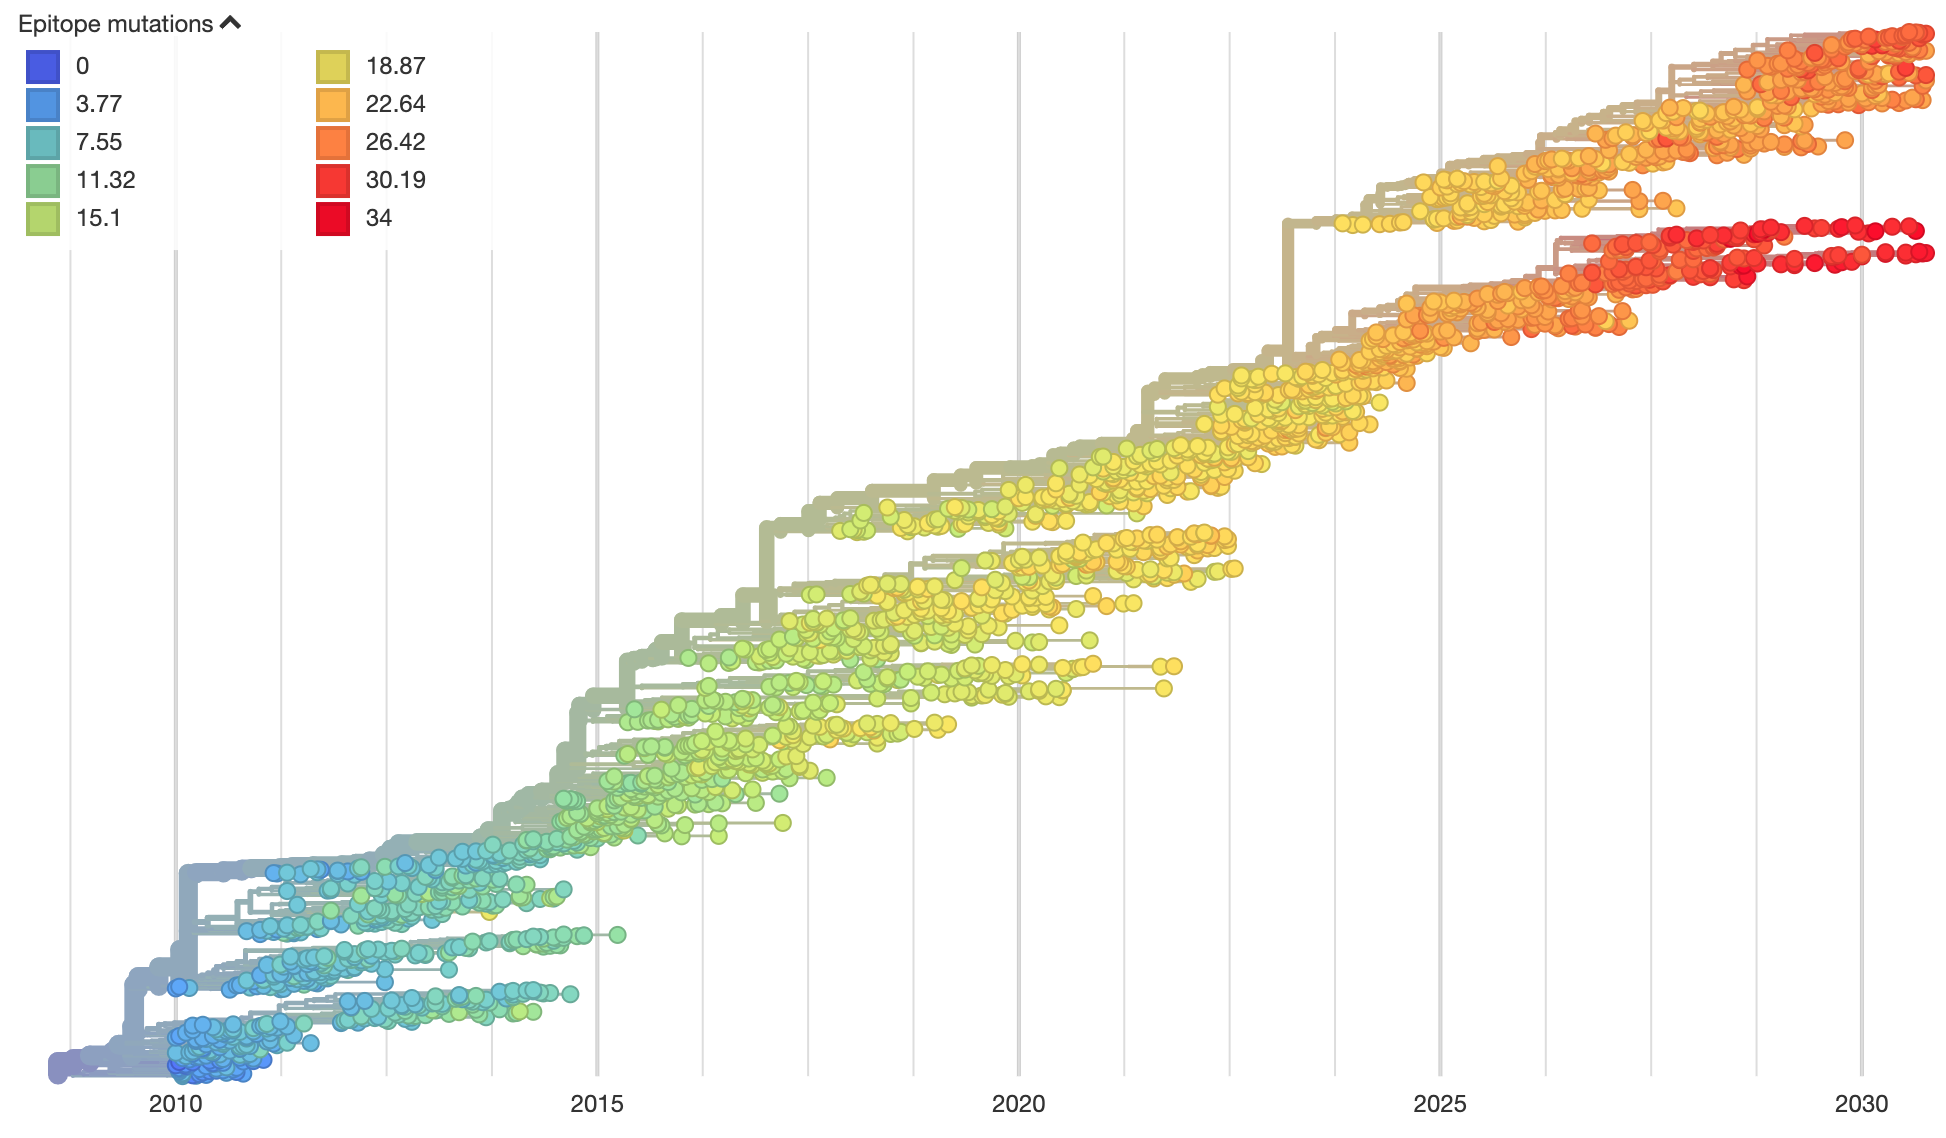
\includegraphics[width=\textwidth]{figures/simulated-h3n2-ha-phylogeny.png}
  \caption{
  Phylogeny of A/H3N2-like HA sequences sampled between the 24th and 30th years of simulated evolution.
  The phylogenetic structure and rate of accumulated epitope and non-epitope mutations match patterns observed in phylogenies of natural sequences.
  Sample dates were annotated as the generation in the simulation divided by 200 and added to 2000, to acquire realistic date ranges that were compatible with our modeling machinery.
  }
  \label{sup_fig:simulated_h3n2_ha_phylogeny}
  \end{center}
\end{figure*}

\begin{figure*}[t]
  \begin{center}
  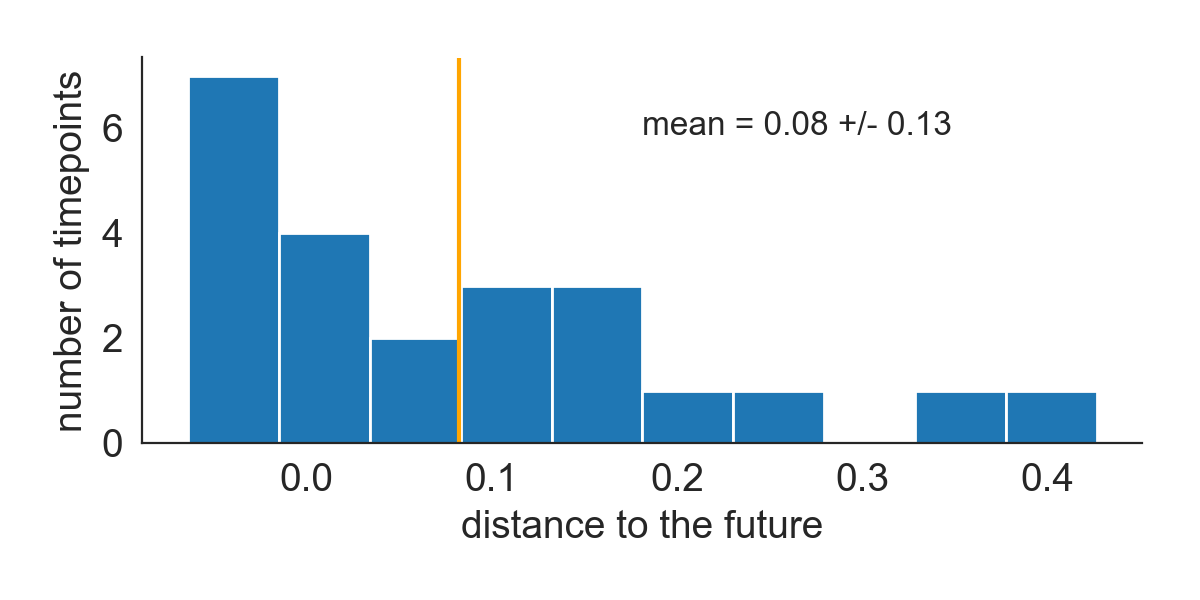
\includegraphics[width=\textwidth]{figures/distance-of-simulated-populations-between-timepoints.png}
  \caption{Average weighted distance per year between simulated populations of viruses under the ``naive'' model.}
  \label{sup_fig:distance_of_simulated_populations_between_timepoints}
  \end{center}
\end{figure*}

\begin{figure*}[t]
  \begin{center}
  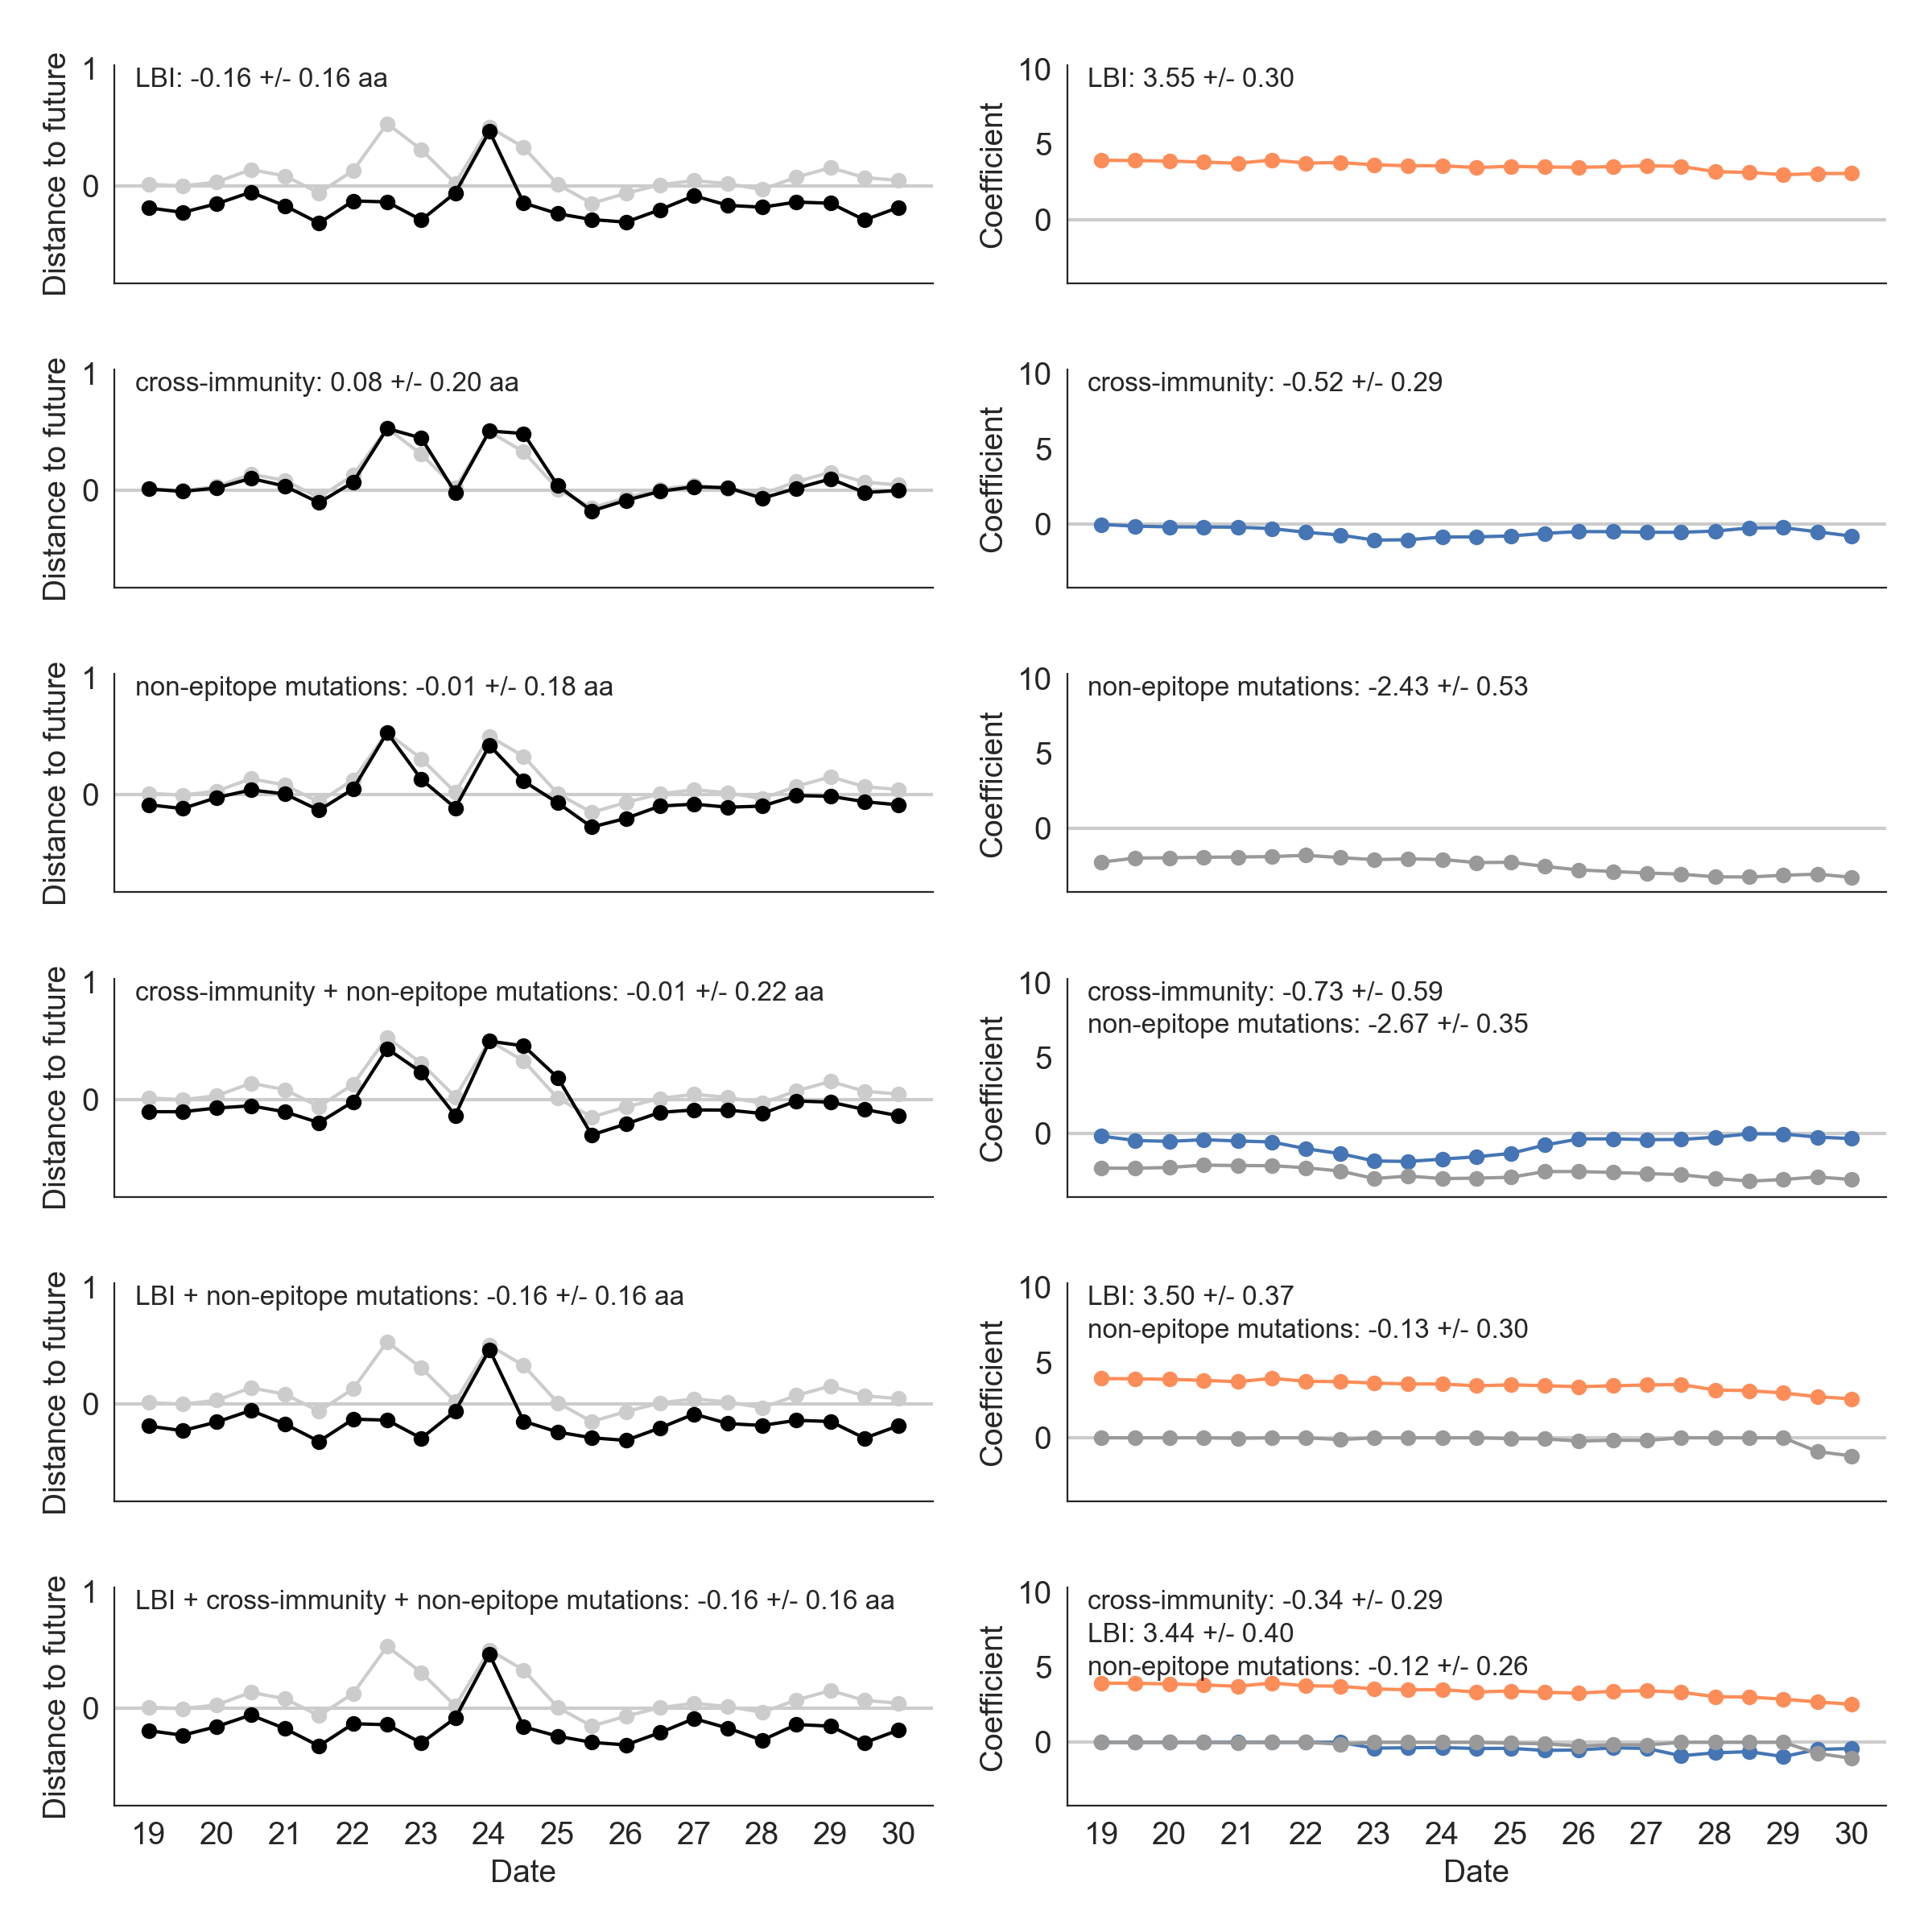
\includegraphics[width=\textwidth]{figures/unadjusted-composite-model-accuracy-and-coefficients-for-simulated-populations.png}
  \caption{Composite model a) accuracy and b) coefficients for simulated populations of A/H3N2-like viruses.}
  \label{sup_fig:unadjusted_composite_model_accuracy_and_coefficients_for_simulated_populations}
  \end{center}
\end{figure*}

\begin{figure*}[t]
  \begin{center}
  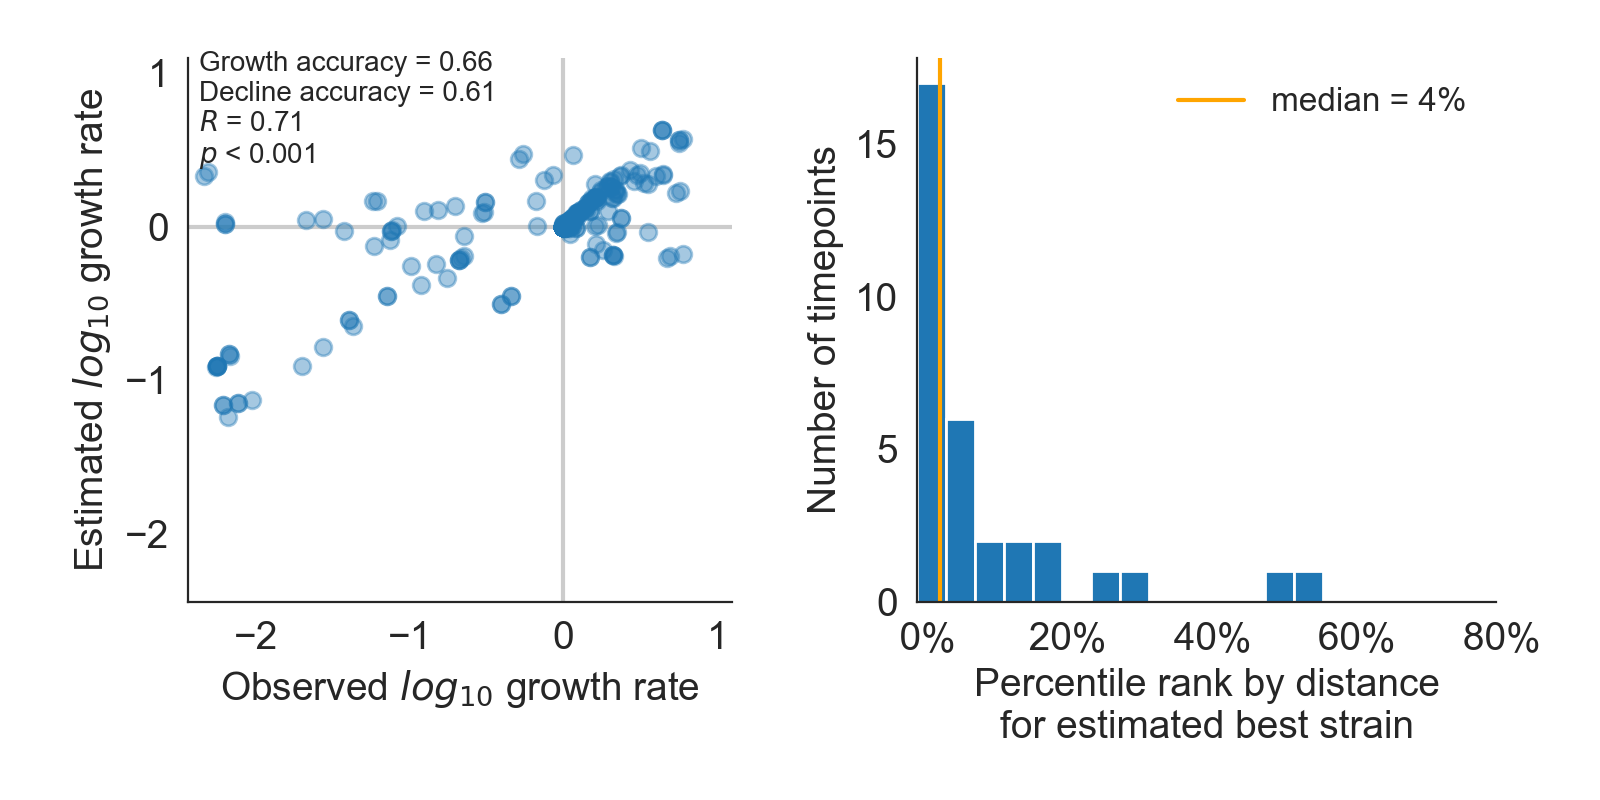
\includegraphics[width=\textwidth]{figures/validation-of-best-model-for-simulated-populations.png}
  \caption{
  Validation of best model for simulated populations of A/H3N2-like viruses.
  a) The correlation of estimated and observed clade growth rates shows the model's ability to capture clade-level dynamics without explicitly optimizing for clade frequency targets.
  b) The rank of the estimated best strain based on its distance to the future in the best model shows how often the model makes a good choice when forced to select a single representative strain for the future population.
  }
  \label{sup_fig:validation_of_best_model_for_simulated_populations}
  \end{center}
\end{figure*}

\begin{figure*}[t]
  \begin{center}
  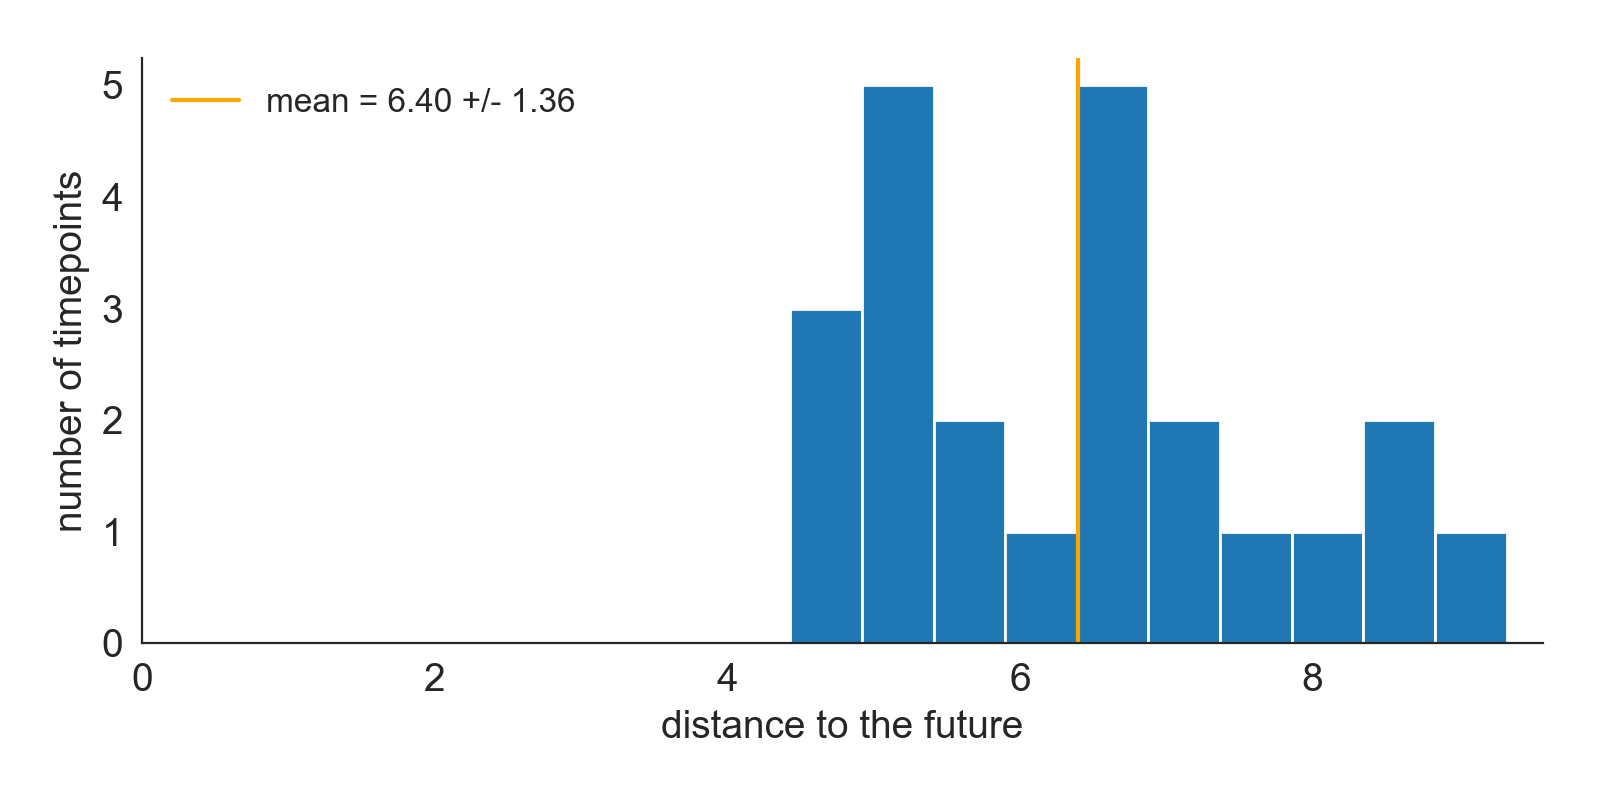
\includegraphics[width=\textwidth]{figures/distance-of-natural-populations-between-timepoints.png}
  \caption{Average weighted distance per year between natural populations of viruses under the ``naive'' model.}
  \label{sup_fig:distance_of_natural_populations_between_timepoints}
  \end{center}
\end{figure*}

\begin{figure*}[t]
  \begin{center}
  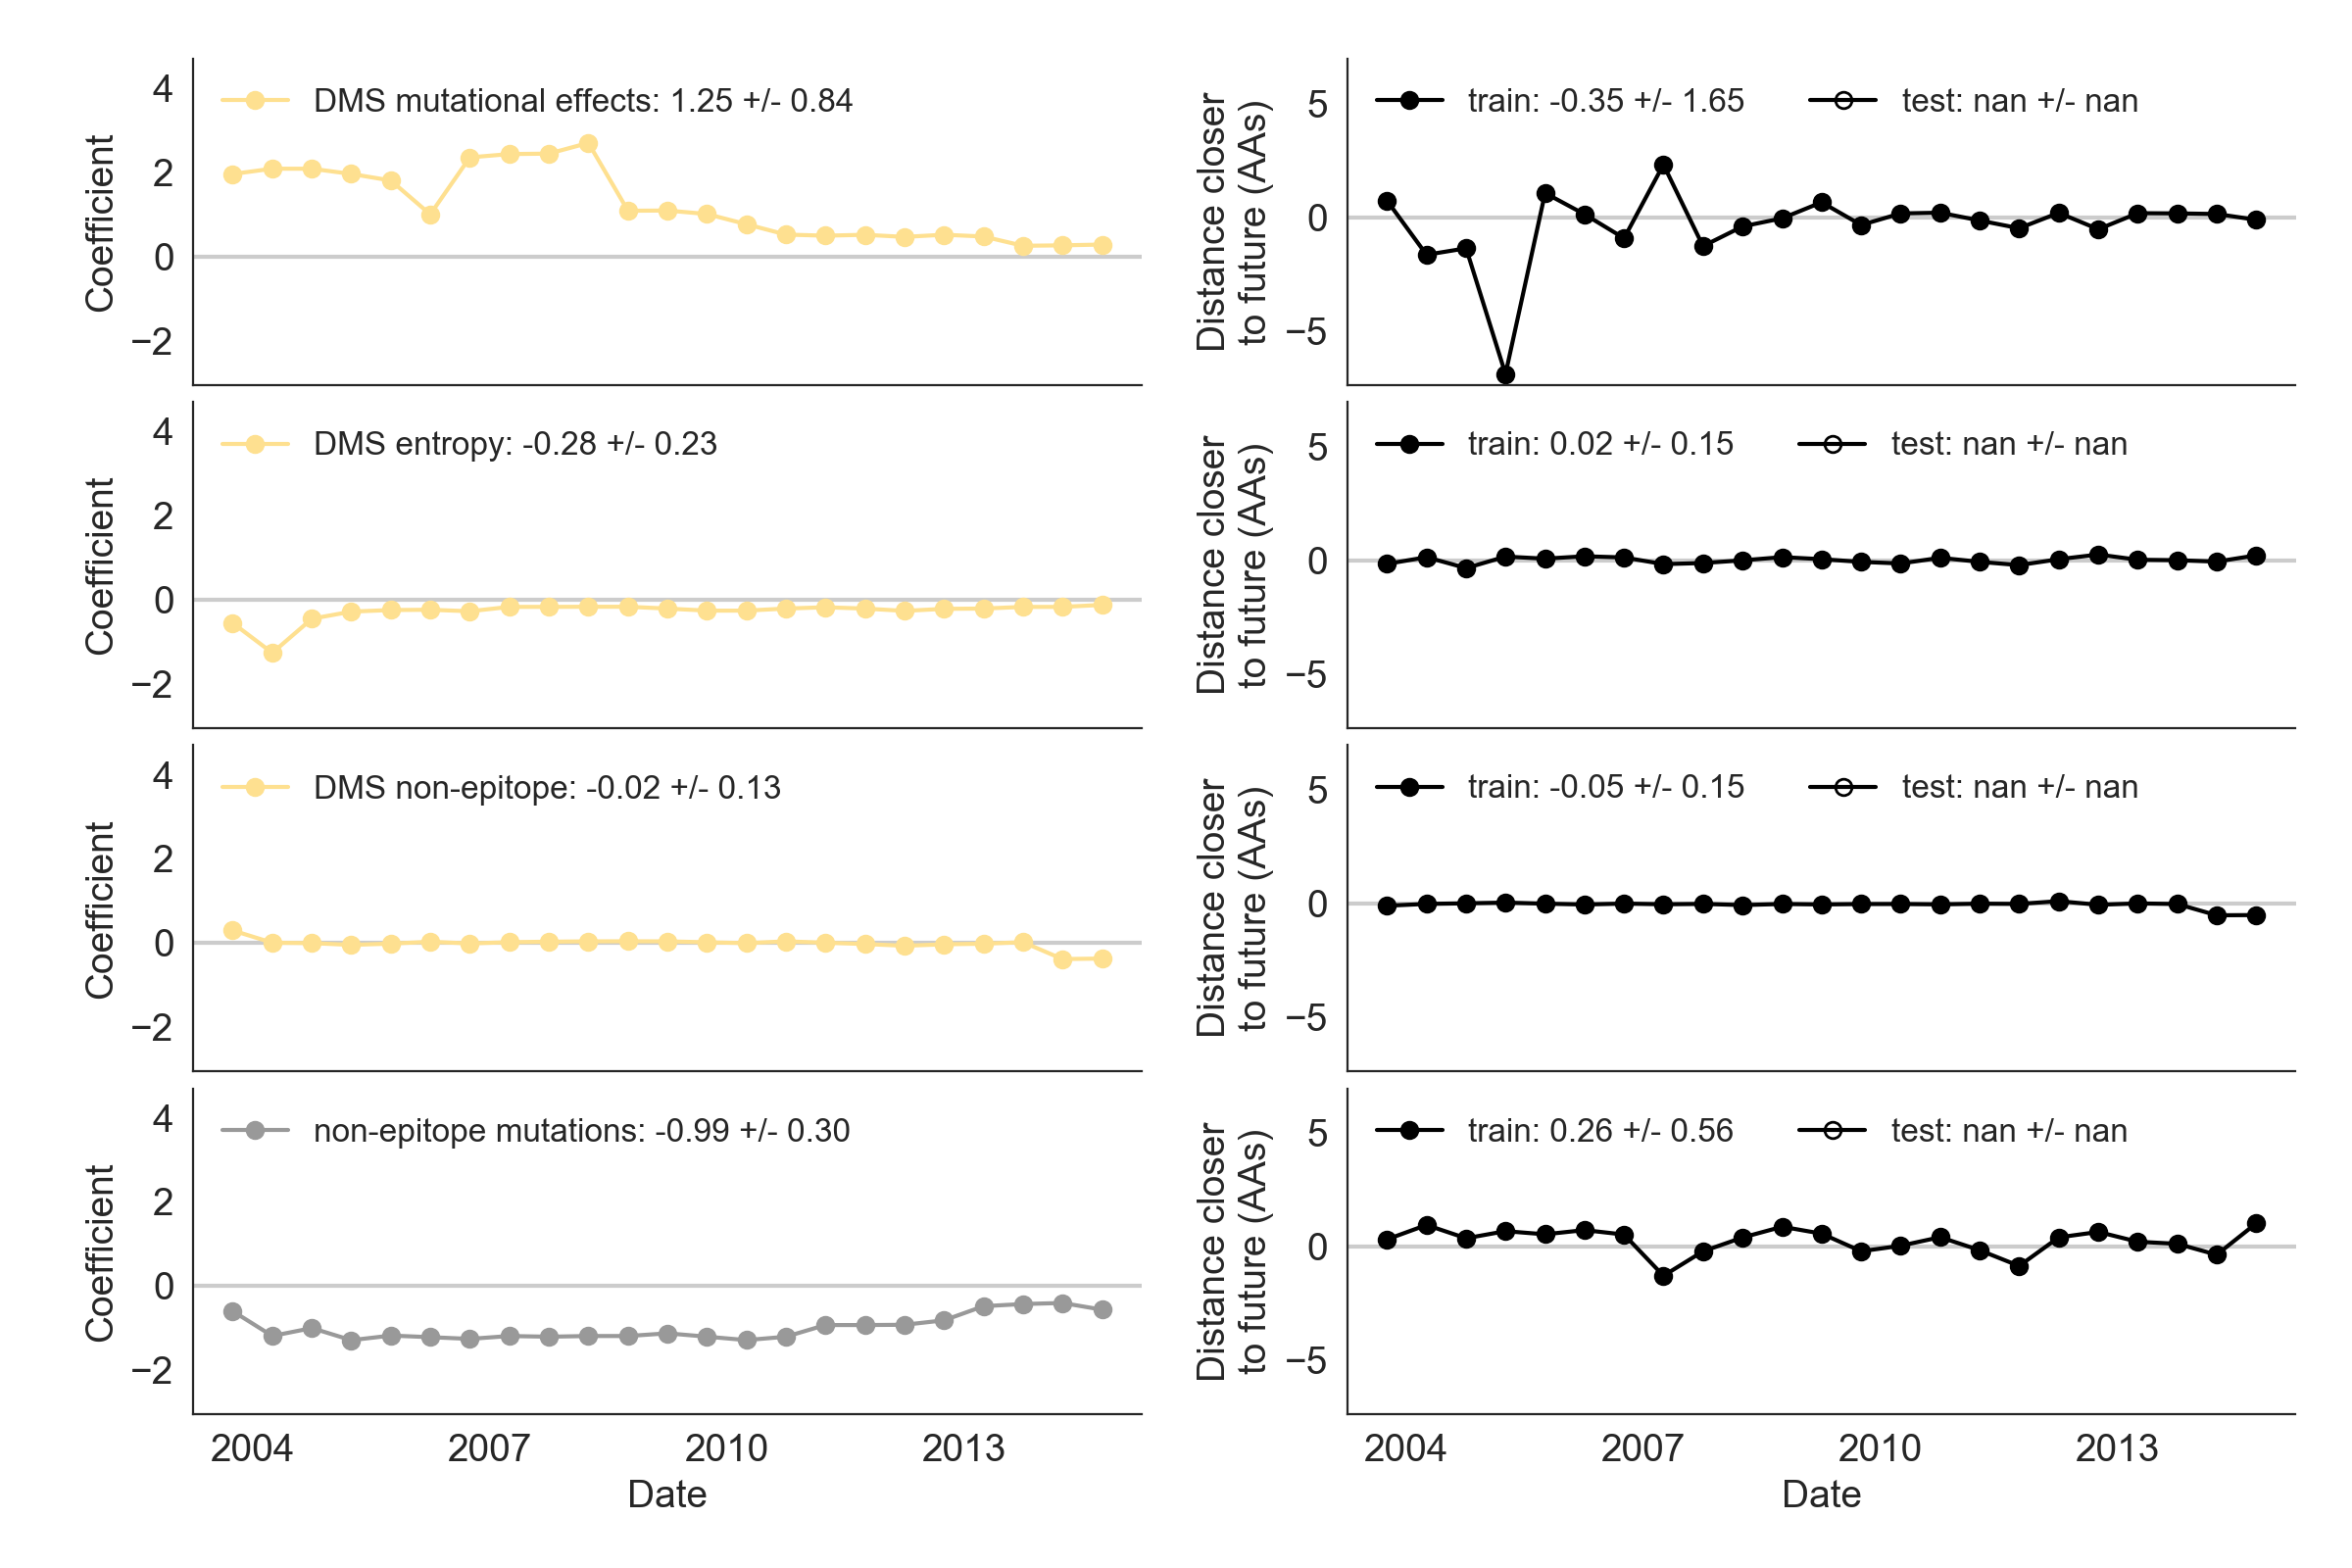
\includegraphics[width=\textwidth]{figures/unadjusted-DMS-model-accuracy-and-coefficients-for-natural-populations.png}
  \caption{
  Primary and alternate fitness metrics based on deep mutational scanning (DMS) preferences for seasonal influenza A/H3N2 strain A/Perth/16/2009.
  Metrics are increasingly less dependent on the sequence content of the DMS strain's genetic background from top to bottom.
  The most structurally naive metric of non-epitope mutations outperforms all of the DMS metrics, indicating that these metrics still overfit to the DMS strain's genetic background.
  }
  \label{sup_fig:unadjusted_DMS_model_accuracy_and_coefficients_for_natural_populations}
  \end{center}
\end{figure*}
